\chapter{Methodology, Comparison, and Technical Analysis of the Base Paper}
\label{chap:comparison}

This chapter provides an in-depth analysis of the base paper, \textit{“Scaling Up the Transformers: A Survey of Training and Inference Optimization Techniques”} by Jahangir et al. (2024), alongside a comparative and methodological examination of the four related works reviewed earlier.  
The discussion is structured into three major parts:
\begin{enumerate}
    \item Methodology of the base paper — detailing how optimization techniques are systematically categorized and analyzed.
    \item Comparative analysis — relating the base paper’s unified framework to other transformer research directions.
    \item Technical insights — highlighting the architectural, algorithmic, and computational implications of these optimization strategies.
\end{enumerate}

This multifaceted exploration not only contrasts the scope and approach of each work but also establishes how these techniques collectively drive the evolution of efficient and intelligent NLP systems.

\newpage

\section{Methodology of the Base Paper}

Jahangir et al. (2024) present one of the most comprehensive surveys of transformer optimization, focusing on both \textbf{training efficiency} and \textbf{inference acceleration}.  
The methodology of their study is divided into three stages — data collection, categorization of techniques, and evaluation synthesis — each designed to systematize and correlate innovations across hundreds of transformer papers.

\subsection{Research Scope and Categorization}
The base paper adopts a hierarchical methodology where optimization is segmented into four major layers:
\begin{itemize}
    \item \textbf{Algorithmic Optimization:} Techniques such as gradient clipping, mixed precision, adaptive learning-rate schedules, and distributed optimizers (e.g., Adafactor, AdamW).
    \item \textbf{Architectural Optimization:} Design-level improvements including parameter sharing, sparse attention, reversible layers, and depth scaling.
    \item \textbf{Training Optimization:} Strategies such as data augmentation, progressive training, and pre-training with regularization.
    \item \textbf{Inference Optimization:} Model compression (quantization, pruning, distillation), caching mechanisms, and hardware–software co-design.
\end{itemize}

Each optimization technique is examined not in isolation but in terms of its contribution to overall model scalability, energy efficiency, and latency reduction.

\subsection{Data Analysis Framework}
The authors use a comparative, metrics-driven framework that evaluates:
\[
\text{Performance Efficiency Ratio (PER)} = \frac{\text{Accuracy Gain}}{\text{Training Cost} + \text{Inference Cost}}
\]
This ratio allows normalization of models with varying resource footprints, providing a unified metric for comparing optimization trade-offs across domains.  
Additionally, the paper introduces visualization matrices comparing methods in terms of:
\begin{itemize}
    \item \textit{Throughput versus Energy Efficiency}
    \item \textit{Latency versus Accuracy Retention}
    \item \textit{Parameter Reduction versus Speedup Ratio}
\end{itemize}
Such multi-dimensional benchmarking allows for identifying not just the best-performing techniques, but also those achieving optimal efficiency–accuracy balance.

\subsection{Survey Methodology and Inclusion Criteria}
The paper analyzes over 100 transformer-related publications, selected based on:
\begin{itemize}
    \item Relevance to training or inference optimization.
    \item Empirical evaluation on standard NLP or vision datasets.
    \item Explicit discussion of performance metrics such as FLOPs, latency, and energy usage.
\end{itemize}
This ensures that the conclusions drawn are representative and empirically validated.

\subsection{Analytical Synthesis}
After compiling experimental results, Jahangir et al. synthesize optimization outcomes through:
\[
\text{Efficiency Gain} = \frac{T_b - T_o}{T_b}
\quad \text{and} \quad
\text{Accuracy Retention} = \frac{A_o}{A_b} \times 100
\]
where \(T_b\) and \(A_b\) are the baseline training time and accuracy, and \(T_o\) and \(A_o\) represent the optimized model’s performance.  
This allows quantification of trade-offs—such as how much training time is saved per percentage point of accuracy loss—thus supporting a balanced assessment.

\newpage
\section{Comparison of Base Paper with Reviewed Works}

\subsection{Comparison with Yenduri et al. (2024) – GPT Review}
Yenduri et al. (2024) focus on the evolution and scaling laws of the GPT architecture, documenting its growth from GPT-1 to GPT-4.  
While their work provides a deep generative overview, it lacks systematic exploration of optimization metrics.

In contrast, Jahangir et al. emphasize scalability through efficiency — framing model growth as a multi-objective optimization rather than mere parameter expansion.

\textbf{Key Comparative Insights:}
\begin{itemize}
    \item Yenduri et al. center on cognitive emergence and language understanding; Jahangir et al. focus on energy-aware computation and real-time deployment.
    \item The GPT review discusses scaling in terms of emergent capabilities; the base paper discusses scaling in terms of computational sustainability.
    \item Jahangir et al. introduce mathematical frameworks linking parameter count to latency and energy cost — an analytical depth absent in the GPT survey.
\end{itemize}

Overall, the base paper serves as a bridge between the theoretical scaling of GPT and the practical engineering needed for deploying such large models efficiently.

\subsection{Comparison with Ur Rahman et al. (2023) – Quantized Transformers}
Ur Rahman et al. (2023) provide one of the most application-oriented studies, focusing specifically on quantization for edge deployment.  
Their empirical approach complements the broader theoretical framework of Jahangir et al. (2024).

\textbf{Comparative Discussion:}
\begin{itemize}
    \item \textit{Granularity:} Ur Rahman et al. operate at the bit-level, analyzing precision trade-offs (e.g., FP32 → INT8). Jahangir et al. incorporate quantization within a layered optimization taxonomy.
    \item \textit{Hardware Correlation:} Both papers connect optimization to physical hardware limits; however, Jahangir et al. integrate it with distributed training and mixed precision pipelines.
    \item \textit{Metricization:} Jahangir’s framework introduces the notion of total energy–accuracy trade-off curves, enabling quantitative assessment across hardware configurations.
\end{itemize}

\begin{figure}[h!]
\centering
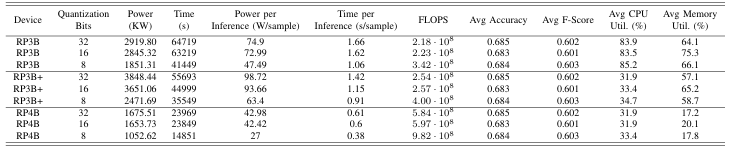
\includegraphics[width=0.8\textwidth]{images/comparison_quantization_flow.png}
\caption{Quantization in edge transformers (Ur Rahman et al., 2023) versus multi-layer optimization strategy (Jahangir et al., 2024).}
\end{figure}

This comparison shows that the base paper transcends device-level optimization to propose a scalable philosophy for transformer efficiency, applicable from edge to cloud-scale systems.

\newpage
\subsection{Comparison with Sanh et al. (2019) – DistilBERT}
Sanh et al. (2019) pioneered model distillation for transformers, creating smaller, faster versions of BERT that retain over 95\% of its performance.  
Their work stands as an early proof of concept for efficiency-centric NLP.  
Jahangir et al. position this within a larger optimization spectrum that unites distillation, quantization, and pruning under one theoretical umbrella.

\textbf{Comparative Analysis:}
\begin{itemize}
    \item Sanh et al. focus exclusively on the teacher–student paradigm. Jahangir et al. extend it by incorporating multi-stage distillation where the student iteratively refines through self-supervision.
    \item The base paper formalizes the distillation loss function into a multi-term efficiency objective:
    \[
    \mathcal{L}_{\text{opt}} = \lambda_1 \mathcal{L}_{\text{CE}} + \lambda_2 \mathcal{L}_{\text{KLD}} + \lambda_3 \mathcal{L}_{\text{speedup}}
    \]
    where each weight factor \(\lambda_i\) balances accuracy and speed.
    \item Sanh’s implementation is task-oriented (GLUE benchmark), while Jahangir’s framework generalizes to multi-domain NLP and CV workloads.
\end{itemize}

\begin{figure}[h!]
\centering
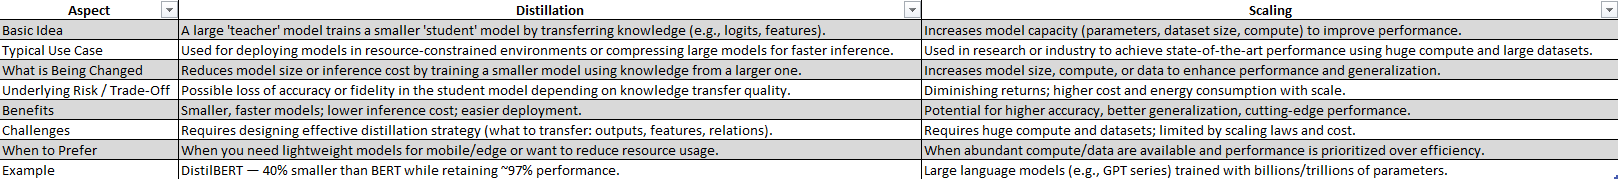
\includegraphics[width=1\textwidth]{images/comparison_distillation_vs_scaling.png}
\caption{Distillation process (Sanh et al., 2019) versus multi-layer unified optimization (Jahangir et al., 2024).}
\end{figure}

Hence, the base paper effectively transforms the concept of distillation from a single technique into part of a unified, sustainable AI framework.

\subsection{Comparison with Azizah et al. (2023) – Transformer Efficiency in Fake News Detection}
Azizah et al. (2023) perform a comparative fine-tuning analysis of BERT, ALBERT, and RoBERTa for fake news detection.  
Their goal is to determine task-level accuracy and computational efficiency across model variants.

While their research is domain-specific, Jahangir et al. elevate this analysis to a system-wide context — explaining how optimization principles improve performance across *all* tasks.

\textbf{Technical Comparison:}
\begin{itemize}
    \item Azizah et al. empirically observe efficiency through runtime and F1-score. Jahangir et al. model it analytically using normalized cost functions for FLOPs and memory.
    \item The base paper introduces Pareto frontiers for optimization trade-offs, while Azizah et al. rely solely on point-based accuracy measurements.
    \item Both works emphasize the importance of architecture-level efficiency; however, Jahangir et al. integrate it with hardware-aware scaling for production environments.
\end{itemize}

\begin{figure}[h!]
\centering
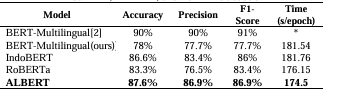
\includegraphics[width=0.8\textwidth]{images/comparison_task_vs_architecture.png}
\caption{Performance comparison of BERT, ALBERT, and RoBERTa versus system-level optimization focus of Jahangir et al. (2024).}
\end{figure}

\newpage
\section{Tabular Comparison of Reviewed Works}

To consolidate these relationships, Table~\ref{tab:comparison} summarizes the methodological and technical distinctions between the reviewed literature and the base paper.

\begin{table}[h!]
\centering
\caption{Methodological and Technical Comparison of Transformer-Based Studies}
\label{tab:comparison}
\begin{tabular}{|p{3cm}|p{2cm}|p{3.5cm}|p{3cm}|p{3cm}|}
\hline
\textbf{Paper} & \textbf{Year} & \textbf{Primary Objective} & \textbf{Optimization / Model Focus} & \textbf{Contribution Level} \\ \hline
Yenduri et al. (GPT Review) & 2024 & Evolution and scaling of generative transformers & GPT (1–4), RLHF, autoregressive training & Cognitive modeling, generative scaling \\ \hline
Ur Rahman et al. (Quantized Transformers) & 2023 & Edge deployment via model compression & Quantization (PTQ, QAT) & Hardware-aware optimization \\ \hline
Sanh et al. (DistilBERT) & 2019 & Compress BERT while maintaining accuracy & Teacher–student distillation & Model-level optimization \\ \hline
Azizah et al. (Transformer Comparison) & 2023 & Evaluate transformer variants for classification & BERT, ALBERT, RoBERTa & Task-level efficiency analysis \\ \hline
Jahangir et al. (Base Paper) & 2024 & Unified optimization of training and inference & Quantization, pruning, mixed precision, parallelism & System-level optimization framework \\ \hline
\end{tabular}
\end{table}

\newpage
\section{Technical Analysis of the Base Paper}

The technical contributions of Jahangir et al. (2024) extend beyond review synthesis—they propose a layered optimization model that redefines how transformers are trained and deployed.

\subsection{Training Optimization Framework}
The base paper categorizes training optimization into:
\begin{itemize}
    \item \textbf{Data-Level Optimization:} Dynamic batching, balanced sampling, and noise-aware pre-training.
    \item \textbf{Model-Level Optimization:} Layer pruning, gradient checkpointing, and knowledge distillation.
    \item \textbf{System-Level Optimization:} Hybrid parallelism (data + model + pipeline) and asynchronous gradient updates.
\end{itemize}

Mathematically, the training time reduction is represented as:
\[
T_{\text{opt}} = T_{\text{base}} \left( \frac{1}{p_d + p_m + p_s} \right)
\]
where \(p_d, p_m, p_s\) denote optimization contributions from data, model, and system levels respectively.

\begin{figure}[h!]
\centering
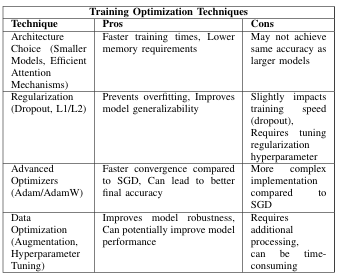
\includegraphics[width=0.9\textwidth]{images/base_training_table.png}
\caption{Training optimization techniques improving efficiency and convergence stability \cite{jahangir2024}.}
\end{figure}

\subsection{Inference Optimization and Acceleration}
Inference optimization focuses on post-training improvements such as pruning redundant weights, quantizing activations, and parallelizing inference pipelines.

\[
S_{\text{speedup}} = \frac{t_{\text{baseline}}}{t_{\text{optimized}}}
\quad \text{and} \quad
A_{\text{retention}} = \frac{Acc_{\text{opt}}}{Acc_{\text{baseline}}}
\]
Together, these define the overall inference performance gain.  

\begin{figure}[h!]
\centering
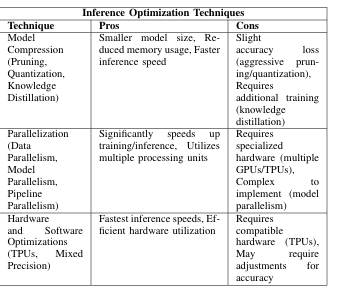
\includegraphics[width=0.9\textwidth]{images/base_inference_table.png}
\caption{Comparison of inference optimization techniques in Jahangir et al. (2024).}
\end{figure}

\subsection{Gradient and Regularization Analysis}
Gradient analysis in the base paper visualizes how different optimizers stabilize training variance.  
Figure~\ref{fig:gradients} shows how Adam variants normalize gradient magnitudes across training steps.

\begin{figure}[h!]
\centering
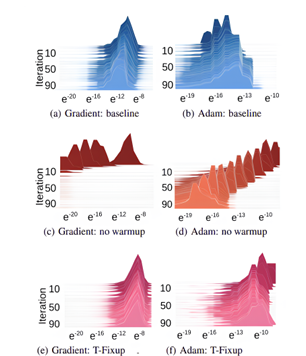
\includegraphics[width=0.9\textwidth]{images/base_gradients.png}
\caption{Gradient stability achieved by adaptive learning-rate optimizers \cite{jahangir2024}.}
\label{fig:gradients}
\end{figure}

These analyses validate that improved normalization and initialization directly translate to faster, more stable convergence.

\subsection{Accuracy–Efficiency Trade-offs}
The base paper’s final analysis examines how optimization affects accuracy using data augmentation and regularization.  
They find that efficient optimization can achieve comparable results to large-scale pre-training, as shown below.

\begin{figure}[h!]
\centering
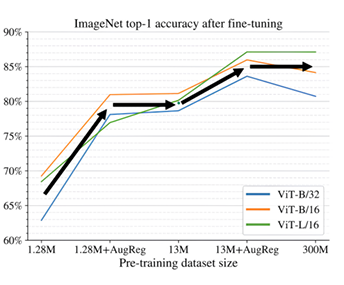
\includegraphics[width=0.9\textwidth]{images/base_accuracy_graph.png}
\caption{Effect of regularization and augmentation on fine-tuning accuracy \cite{jahangir2024}.}
\end{figure}

This demonstrates that intelligent optimization can substitute brute-force scaling, achieving sustainable AI without exponential compute growth.

\newpage
\section{Summary}

The methodological, comparative, and technical analysis shows that:
\begin{itemize}
    \item The base paper unifies the fragmented research on transformer optimization into a layered, holistic framework.
    \item It quantitatively connects efficiency and accuracy, unlike earlier qualitative surveys.
    \item Compared to task-specific or model-specific works (GPT, Quantization, Distillation, Fake News Detection), it generalizes principles applicable across domains.
\end{itemize}

Ultimately, Jahangir et al. (2024) redefine transformer research by integrating training and inference optimization into a single, sustainable paradigm.  
This systematic approach not only enhances performance but also establishes the foundation for scalable, human-centered AI architectures.
